\scanpage{131}
\mspage{V.2}
% archive sheet number: 130

% L01-02 left upper margin, pencilled and slanted
% margin note written slanted
\margin{\figure{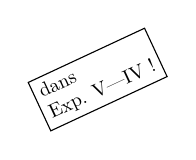
\begin{tikzpicture}[scale=.7,transform shape]
\node[draw,rotate=25,align=left] {dans\\ Exp. \unsure{V|IV} !};
\end{tikzpicture}}}

% L01-06
\deleted{\unsure{1.4}}1.1. Nous allons donner une interprétation frappante des fibres $(\underline{\Psi}_{\unsure{\alpha|\nu}}^{(q)})_{\overline{x}}$ des faisceaux introduits dans (\inserted{\uline{III}} 2.6), où $\overline{x}$ est un point géométrique de $\widetilde{X}_0$. Pour ceci, introduisons le localisé strict $\overset{\deleted{\unsure{\sim}}}{X}'$ de $\widetilde{X}$ en $\overline{x}$; \deleted{\unsure{et}}\inserted{nous pouvons \unsure{identifier}} le localisé strict correspondant de $S$ égal à $\widetilde{S}$, du fait qu'on a un morphisme canonique

% L05 margin enclosed in a box
\margin{\figure{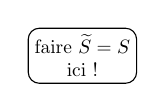
\begin{tikzpicture}[scale=.7,transform shape]
\node[draw,rounded corners,align=center] {faire $\widetilde{S}=S$\\ ici !};
\end{tikzpicture}}}

% L07
\[
\overset{\deleted{\sim}}{f}' : \overset{\deleted{\sim}}{X}'\longrightarrow\widetilde{S}
\tag*{\deleted{\unsure{(0.1.1)}} (1.1.1)}
\]

% L08-10
Si $\overset{\deleted{\sim}}{U}'$ est l'image inverse de $U$ dans $\overset{\deleted{\sim}}{X}'$, c'est un ouvert de la fibre générique $\overset{\deleted{\sim}}{X}'_{\widetilde{\eta}}$ de $\overset{\deleted{\sim}}{f}'$ sur $\widetilde{S}$ :
\[
\overset{\deleted{\sim}}{U}'\subset\overset{\deleted{\sim}}{X}'_{\widetilde{\eta}}.
\tag*{\unsure{(1.1.2)}}
\]

% L11-12
Ceci posé, le \deleted{\unsure{calcul du}} calcul habituel des fibres de faisceaux \inserted{$R^{\unsure{q|i}}g_*$} (SGA 4 \uline{VIII}\quad) montre qu'on a

% L13 bottom left margin, slanted and enclosed
% margin note written slanted
\margin{\figure{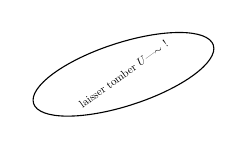
\begin{tikzpicture}[scale=.4,transform shape,rotate=18]
\draw (0,0) ellipse (3cm and 1cm);
\node[rotate=18] at (0,0) {laisser tomber \unsure{$U$|$\sim$} !};
\end{tikzpicture}}}
